\chapter{Filtrering af signal}
I dette kapitel designes et båndstopfilter med endelig impulsrespons (altså et FIR-filter), der har til formål at eliminere den midterste frekvens ved $\omega_2 = \frac{\pi}{2}$ mest muligt og samtidig reducere de øvrige frekvenser ved $\omega_1 = \frac{\pi}{3}$ og $\omega_3 = \frac{3\pi}{4}$ mindst muligt. I kapitlet beskrives først specifikationerne og design af filteret, hvorefter filterets effekt på signalet vurderes. Afslutningsvist forsøges filteret optimeret.
\section{Specifikationer} \label{ch4_specs}
FIR-filteret vælges til at være af type 1, altså er filterordenen $M$ lige og impulsresponsen $h[n]$ er symmetrisk, så $h[n] = h[M - n]$. Filteret har 2 knækfrekvenser $\omega_{c_1}$ og $\omega_{c_2}$ i rad/s, som vælges til at ligge symmetrisk omkring $\omega_2$, der skal elimineres ved hjælp af filteret:
\begin{align*}
\omega_{c_1} &= \omega_2 - \delta, \\
\omega_{c_2} &= \omega_2 + \delta,
\end{align*}

hvor $\delta$ vælges til at være $\frac{\pi}{15}$. Filteret designes dermed som et båndstopfilter med ovenstående knækfrekvenser. Den ideelle amplituderespons $H_d(\text{e}^{j\omega})$ er skitseret på figur \ref{fig:ideel_amp_respons} ud fra de opstillede specifikationer.   
\begin{figure}[H]
    \centering
    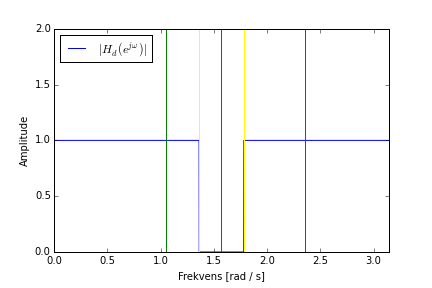
\includegraphics[width = 0.6\textwidth]{figures/ideel_amp_respons.PNG}
    \caption{Den ideelle amplituderespons for filteret. De to grønne streger markerer $\omega_1$ og $\omega_3$, som skal beholdes, og de to gule streger markerer $\omega_{c_1}$ og $\omega_{c_2}$, som ligger symmetrisk omkring den røde streg, der markerer $\omega_2$, som skal elimineres.}
    \label{fig:ideel_amp_respons}
\end{figure}

\section{Design af filter} \label{ch4_design}
I dette afsnit dokumenteres designprocessen samt væsentlige dele af Python-koden, der anvendes til at filtrere signalet.\\
Først defineres henholdsvis filterordenen $M$, længden af filteret $l = M + 1$, en vektor $n$ med $l+1$ heltal mellem 0 og $l$ samt en vektor $x$ med $l+1$ værdier mellem $-\pi$ og $\pi$.
\\ \\
Den ideelle impulsrespons $h_d$ defineres nu som en funktion på baggrund af den ideelle amplituderespons $|H_d(\text{e}^{j\omega})|$, jf. figur \ref{fig:ideel_amp_respons}. Udledning af $h_d[n]$ findes i bilag \ref{app1}. \\
Funktionen i Python bruger vektoren $n$, ordenen $M$ samt frekvenserne $\omega_{c_1}$ og $\omega_{c_2}$ defineret ovenfor. Den ideelle impulsrespons er derfor:
\begin{align*}
h_d[n] = \begin{cases} \dfrac{\sin\left(\omega_{c_1}\left(n - \frac{M}{2}\right)\right)}{\pi\left(n - \frac{M}{2}\right)} - \dfrac{\sin\left(\omega_{c_2}\left(n - \frac{M}{2}\right)\right)}{\pi\left(n - \frac{M}{2}\right)} \quad &\text{for} \quad n \neq \frac{M}{2} \\
1 - \frac{\omega_{c_2} - \omega_{c_1}}{\pi} \quad &\text{for} \quad n = \frac{M}{2}
\end{cases}
\end{align*}
Dette er implementeret i koden således:
\begin{lstlisting}
def hd(n,M,f1,f2): 
    hd = np.zeros(len(n))
    for i in range(len(n)):
        if n[i] == M/2:
            hd[i] = 1 - (f2 - f1)/np.pi
        else:
            hd[i] = (np.sin(f1*(n[i] - M/2.)) / (np.pi*(n[i] - M/2.))) \
            - (np.sin(f2*(n[i] - M/2.)) / (np.pi*(n[i] - M/2.)))
    return hd
\end{lstlisting}
Fordi impulsresponsen er endelig skal den ideelle impulsrespons ganges med en vinduesfunktion, og dette Fourier-transformeres herefter for at opnå en realiserbar frekvens- og amplituderespons. Der er forskellige muligheder for denne vinduesfunktion såsom det rektangulære vindue, Hamming-vinduet, Hann-vinduet og Blackman-vinduet.$^[$\footnote{Disse vinduer er beskrevet på side 559-560 i \textit{Discrete-Time Signal Processing}, Oppenheim \& Schafer (2014).}$^]$ Implementeringen af vinduerne i koden er ganske simpel, og som eksempel ses implementeringen af Hann- og Hamming-vinduet herunder:
\begin{lstlisting}
def ha(n,M,a): # Hann-vindue, hvis a = 0.5. Hamming-vindue, hvis a = 0.54.
    w = np.zeros(len(n))
    for i in range(len(n)):
        if n[i] >= 0 and n[i] <= M:
            w[i] = a - (1 - a)*np.cos((2*np.pi*n[i])/M)
        else:
            w[i] = 0
    return w
\end{lstlisting}

Hamming-vinduet er vist samplet på figur \ref{fig:Hamming}.
\begin{figure}[H]
    \centering
    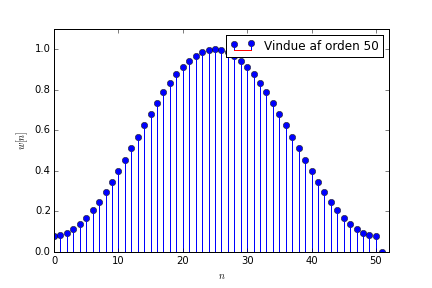
\includegraphics[width = 0.6\textwidth]{figures/Filter/Hamming-vindue.PNG}
    \caption{Eksempel på Hamming-vinduet.}
    \label{fig:Hamming}
\end{figure}

Efter implementeringen af vinduerne kaldes funktionerne for den ideelle impulsrespons og det ønskede vindue, som herefter ganges sammen. Dette resultat Fourier-transformeres ved hjælp af den implementerede FFT beskrevet under frekvensanalysen. Hermed opnås frekvensresponsen $H(\text{e}^{j\omega})$ og amplituderesponsen $|H(\text{e}^{j\omega})|$, hvoraf sidstnævnte (ideelt set) er 0 mellem $\omega_{c_1}$ og $\omega_{c_2}$ og 1 ellers. Dette afhænger dog især af valget af vinduet og filterordenen $M$. Figur \ref{fig:filter_rekt} viser eksempler på anvendelsen af det rektangulære vindue for $M = 30$ og $M = 100$.

\begin{figure}[H]
\begin{minipage}{0.49\textwidth}
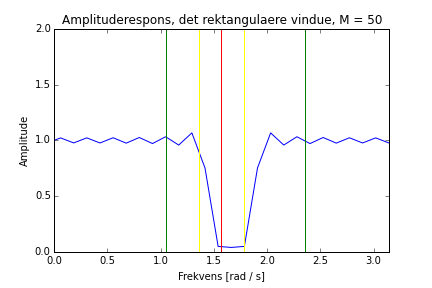
\includegraphics[width=0.9\textwidth]{figures/Filter/Filter_rekt_50.PNG}
\end{minipage}
\begin{minipage}{0.49\textwidth}
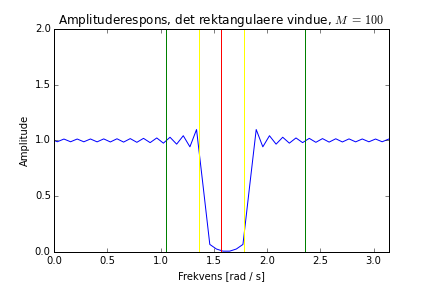
\includegraphics[width=0.9\textwidth]{figures/Filter/Filter_rekt_100.PNG}
\end{minipage}
\caption{Eksempler på båndstopfilteret under anvendelse af det rektangulære vindue og med forskellige filterordener $M$.}
\label{fig:filter_rekt}
\end{figure}

Ud fra figur \ref{fig:filter_rekt} ses det, at filteret til en vis grad overholder specifikationerne for begge værdier af $M$, at transitionsbåndet bliver smallere for højere $M$ samt at der dog er såkaldte ``ripples'' i pasbåndet. Disse ``ripples'' skyldes diskontinuiteterne ved det rektangulære vindue, der pludselig skifter fra $0$ til $1$ og tilbage igen. For at undgå dette kan man bruge et glattere vindue som for eksempel Hamming-vinduet illustreret på figur \ref{fig:Hamming}.
\section{Vurdering}
På bagrung af graferne i sektion \ref{resultater} kan det konkluderes at det designede FIR filter af orden ?? formår at filtrere frekvensen $\omega_2=\frac{\pi}{2}$ fra det samplede signal $s[n]$, som ønsket.\\
Figur \ref{amplitude respons} illustrerer at de opstillede specifikationer til en vis grad overholdes ved en orden på hhv. 30 og 100 og anvendelse af det reksangulare vindue. Dog ses det tydeligt at transitionsbåndet bliver smallere jo højere orden der anvendes. De ripples der forekommer i passbåndet formindske ligeså, som ordnen øges, dog forsvinder de ikke som resultat at at det er det rektangulere vindue der anvendes. Som nævnt kan dette optimeres ved at ændre vinduet, hvilket undersøges nærmere i næste afsnit. \\
Figur \ref{filt signal i frekvens} illustrere yderligere hvorledes den ønskede frekvens er fjernet, uden at fjerne de omkring liggende frekvenser. Dog ses som resultat af de forekommende  rippels i passbåndet at amplituderesponsen på de tilbageværende frekvenser forvrænges en smule.    
Ved sammenligning af amplituderesponsen for det designede filter \ref{?} og den ideelle amplituderespons, skitseret på figur \ref{?}, vurderes det altså at det designede filter kan optimeres yderligere. \\
          
%\section{Optimering}
For at optimere filteret anvendes et andet vindue. Ved at eksperimentere med de forskellige vinduer ses det, at der også opstår ripples ved Blackman-vinduet, hvorimod anvendelser af Hann- og Hamming-vinduet giver ingen eller meget små ripples. Eksempler på dette er vist i figur \ref{fig:filter_Hann_Hamming}.
\begin{figure}[H]
\begin{minipage}{0.49\textwidth}
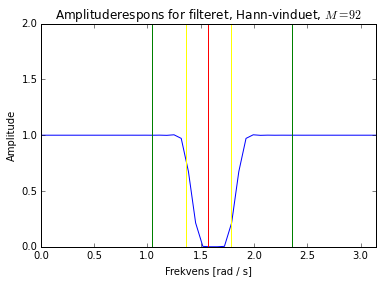
\includegraphics[width=0.9\textwidth]{figures/Filter_Hann_92.PNG}
\end{minipage}
\begin{minipage}{0.49\textwidth}
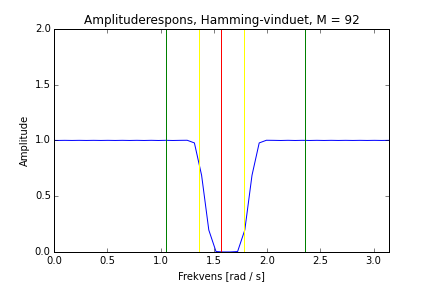
\includegraphics[width=0.9\textwidth]{figures/Filter_Hamming_92.PNG}
\end{minipage}
\caption{Eksempler på båndstopfilteret under anvendelse af Hann- og Hamming-vinduet med $M=92$.}
\label{fig:filter_Hann_Hamming}
\end{figure}

Fra figur \ref{fig:filter_Hann_Hamming} fremgår det, at der ikke er nogle ripples i pasbåndet, hvor amplituden desuden er 1. Derudover er amplituden 0 i stopbåndet, hvor $\omega_2$ ligger. Således opfylder filteret specifikationerne for denne filterorden. Lavere orden medfører færre beregninger og bredere transitionsbånd, og sidstnævnte har ikke nogen særlig betydning i dette tilfælde, fordi afstandene mellem de 3 frekvenser i signalet er så store.
